%! TeX program = lualatex
\documentclass[../main.tex]{subfiles}
\begin{document} \section{Power rule models \texorpdfstring{\(y =  c x^{\alpha}\)}{} and log-log transformation}

Visualization is often a helpful method to \emph{make sense} of data collected from empirical studies.

\begin{definition}[log-log space]
  A point \((x,y)\) in the Euclidean space corresponds to \((\ln(x), \ln(y))\) in the log-log space, and a point \((\alpha,\beta)\) in the log-log space corresponds to \((e^{\alpha}, e^{\beta})\) in the Euclidean space.

  Sometimes, we use the calculator notation \(\exp(\cdots)\) to mean \(e^{\cdots}\).
\end{definition}

\begin{figure}[H] % [h] for here, [ht] for here top, [hb] for here bottom
  \centering
  
  \hfill{}
  \includegraphics{../standalones/build/plot-blank-5x5.pdf}
  \hfill{}
  \includegraphics{../standalones/build/plot-log-log-5x5-plain.pdf}
  \hfill{}

  \caption{Euclidean space vs log-log space.}
  \label{fig:figure}
\end{figure}

\faExclamationTriangle{} Axes labels tell us whether a plot is given in Euclidean or log-log space.

% (e^0, e^2), (e^3, e^4)
\begin{example}
  Consider points \((1,8)\) and \((20, 50)\) in the Euclidean space. Sketch their corresponding points in the log-log space. Use a calculator to approximate \(\ln(\cdots)\) values.

  \blanklines{2}
\end{example}

\begin{example}
  Consider points \((0, 0)\) and \((1.5, 2.3)\) in the log-log space. Sketch their corresponding points in the Euclidean space. Use a calculator to approximate \(\exp(\cdots)\) values. 

  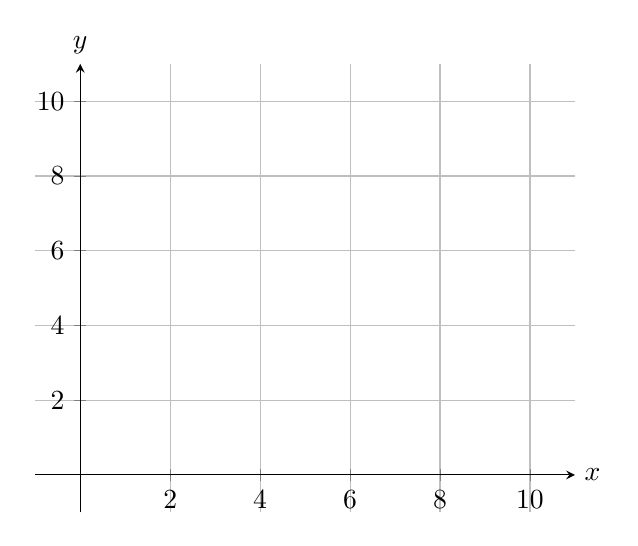
\begin{tikzpicture}
    \begin{axis}[
      xmin=0,ymin=0,xmax=10,ymax=10,
      grid=major,
      axis lines=middle, 
      enlargelimits=true,
      xlabel={\(x\)}, xlabel style={anchor=west},
      ylabel={\(y\)}, ylabel style={anchor=south},
      ]

    \end{axis}
  \end{tikzpicture}
\end{example}

\clearpage
\begin{definition}[log-log transformation]
  The (natural) log-log transformation of an equation \(y = c x^{\alpha}\) is
  \[
    \ln(y) = \ln(c) + \alpha \ln(x)
  \]
  obtained by applying \(\ln(\cdots)\) to both sides of \(y = c x^{\alpha}\).
\end{definition}

\blanklines{3}

\begin{example}[warm-up]
  Sketch the model \(y = 0.135 (\sqrt{x})^{3}\) in the log-log space. 

  Takeaway: A power rule model \(y = c x^{\alpha}\) appears as a \underline{\hspace{2in}} in log-log space.

  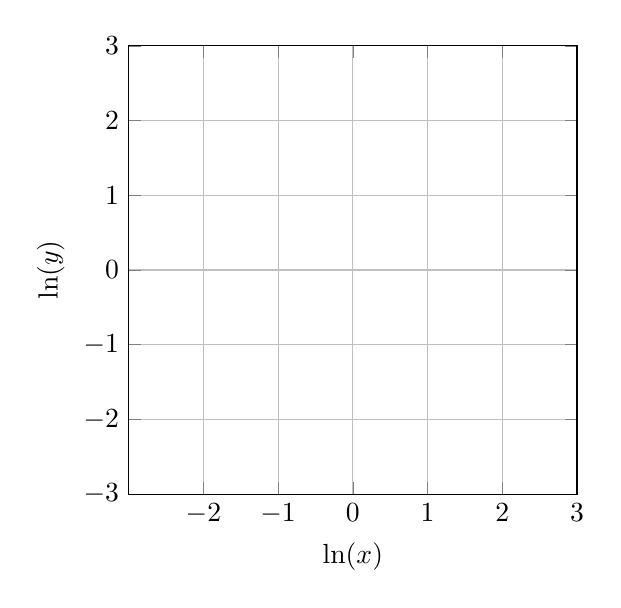
\begin{tikzpicture}
    \begin{axis}[
      axis equal image,
      ylabel={\(\ln(y)\)},
      xlabel={\(\ln(x)\)}, 
      xmin={-3},xmax={3},
      ymin={-3},ymax={3},
      xtick={-2,...,3},ytick={-5,...,3},
      grid=major,
      ]
    \end{axis}
  \end{tikzpicture}

\end{example}

\faStar{} The following describes \hlmain{the theory underlying applications} of log-log transformation of \(y = c x^{\alpha}\).

We are often given data in Euclidean spaces.  Using biology or visual inspection, we suspect a power rule model \(y = c x^{\alpha}\) should fit the data and wish to determine the coefficient \(c\) and the exponent \(\alpha\). We do so by plotting the log-log transformation of our data and figure out a best-fit line \(\ln(y) = C + \alpha \ln(x)\) in the log-log space. We identify its slope to be \underline{\hspace{1in}} and vertical intercept to be \underline{\hspace{1in}}. Finally, we apply \(\exp(\cdots)\) to both sides of \(\ln(y) = C + \alpha \ln(x)\) to recover the desired model.

\includegraphics{../standalones/build/plot-log-log-5x5-plain.pdf}

In the following example, we practise performing the last step of an application of log-log transformation, i.e., identify a model \(y = c x^{\alpha}\) from its log-log transformation. 

\begin{example}
  The log-log transformation of a model \(y = c x^{\alpha}\) is sketched below.  Identify the model, i.e., figure out \(c\) and \(\alpha\) and write down the equation of the model. 

  Approximate all numbers to three decimal places.

  \includegraphics{../standalones/build/plot-log-log-example.pdf}
\end{example}


\bigskip{}

\faCalculator{} Be aware that most online calculators display log-log transformations without transforming the labels of the horizontal and vertical axes. Desmos' built-in log-log transformation does this. \faExclamationTriangle{} In such a case, the \(y\)-intercept you read off \hlsupp{a log-log graph whose axes labels are not transformed} is NOT the \(C\) in \(\ln(y) = C + \alpha \ln(x)\); instead, the \(y\)-intercept you read off such a graph is \(e^{C}\).

\end{document}
